\documentclass[a4paper, 12pt]{article}
% Options possibles : 10pt, 11pt, 12pt (taille de la fonte)
% oneside, twoside (recto simple, recto-verso)
% draft, final (stade de développement)
\usepackage[utf8]{inputenc} % LaTeX, comprends les accents !
\usepackage[T1]{fontenc} % Police contenant les caractères français
\usepackage{geometry} % Définir les marges
\usepackage[francais]{babel} % Placez ici une liste de langues, la
% dernière étant la langue principale
\usepackage{graphicx}
\usepackage{verbatim}
\usepackage{float}
\usepackage{booktabs}
\usepackage{amsmath}
\usepackage{amsfonts}
\usepackage{multirow}
\geometry{left=2.2cm,right=2.2cm,top=2.5cm,bottom=2.5cm}
% \pagestyle{headings} % Pour mettre des entêtes avec les titres
% des sections en haut de page
%\include[dvips]{graphics}
\title{Reinforcement Learning Project Report \\ \vspace{0.5cm} \large Unsupervised and Reinforcement Learning in Neural Networks}
\author{Han JU, Hao REN}
\date{\today}
\begin{document}
\maketitle
\section{Introduction}

In this project we implement a reinforcement learning experiment with
continuous state space and a neural network model. Unlike the discrete
state learning experiments, in a continuous state space we can't
enumerate over all possible states, that makes the classic Q-learning
algorithm not applicable here. Instead, with the help of a neural
network model taught in the course, we are able to code the state
space by a finite number of input neurons, namely the place cells. On
the other side, we have the action cells, each represents an possible
action of the agent in the experiment. Given this set up, the expected
reward for a particular point in the state space is just the dot
product of the point's activation of all place cells and the weight
vector between the place cells and the action cells. So essentially we
use the classic SARSA algorithm's framework, but what we update is the
weight vector, and the Q-values are computed dynamically for choosing
an action.

For the implementation, we adapt it from the given python code in the
exercise session.

\section{Learning curve}

Right after the implementation according to the project set-up, we
begin our experiment by conducting 10 independent runs with 50 trials
each. Figure 1 is the resulting learning curve.

\begin{figure}[h]
\centering
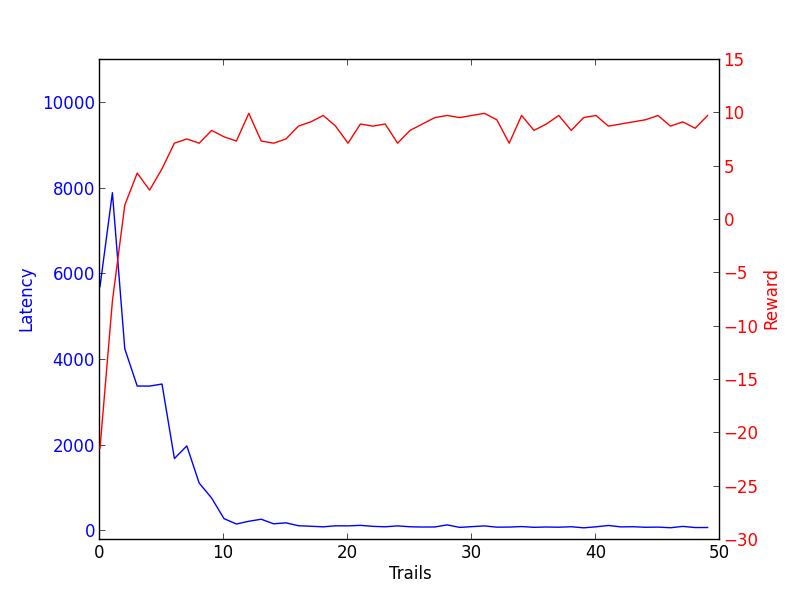
\includegraphics[scale=0.4]{../figure/learning_curve.jpg}
\caption{Learning curve of a complete experiment}
\end{figure}

For this very first experiment, we set the epsilon parameter to $0.5$,
which means half of agent's moves are random. The leaning curve makes
perfect sense: the first several runs are nearly random walks, which
take over 5000 steps thanks to the randomness and the yet not very
effective W-values. However, after several tastes of the goal, due to
the effect of the eligibility trace, this information is quickly
propagated throughout the weight vectors between the input space cells
and the action neurons. As a result, half of the time the agent
chooses the right direction that leads it to the goal area and avoids
the wall hitting, the steps needed are decreasing drastically. We can
observe that within 10 trials, this number goes down from 8000 to
a stable value of aprroximately 100. Note that because of the
randomness, there is some fluctuation on the curve.

As for the average reward, showed in red curve in the figure, it has
generally the same trend as the latency curve. For example in the
first several trials, the agent is essentially exploring the state
space, so it hits often the wall and that causes a very low overall
reward. As the agent's knowledge of the state space grows, its reward
per trial converges to 10, which means it pursues directly the goal
area without hitting too much the wall.

\section{Exploration \& Exploitation}
The parameter $\epsilon$ controls the balance between exploration and exploitation. When $\epsilon$ is big, the agent has more possibilities to take a random step in order to explore more place in the environement, while small $\epsilon$ makes the agent more likely to take a step according to the $\epsilon$-greedy policy. The implementation of the algorithm SARAR depends on the choice of the $\epsilon$, we have to make a tradeoff. If the $\epsilon$ is too big, the agent will seldom take a step with the greedy policy, the whole learning process is more stochastic, so the learning result is not significant. However, if $\epsilon$ is too small, the agent will be more likely to exploit the state around where it is, because the weights are not largely updated, the agent sometimes will travel around several same states, sometimes even not get to the goal within a given time step limit.

The best solution is to start with a big $\epsilon$ so as to explore the space as widely as possible. The $\epsilon$ decreases after each trails Thus, the first several trials with big $\epsilon$ will collect enough information about the weights (Q values), and the later trials with small $\epsilon$ can take a good use of these information via the greedy policy which makes the agent more likely to get into the goal area.

The learning curves and the average latency of the last 10 trails with $\epsilon$=0.8, 0.6, 0.4, 0.2 are shown as below:

\begin{figure}
  \centering
  \begin{minipage}[c]{0.5\textwidth}
    \centering
    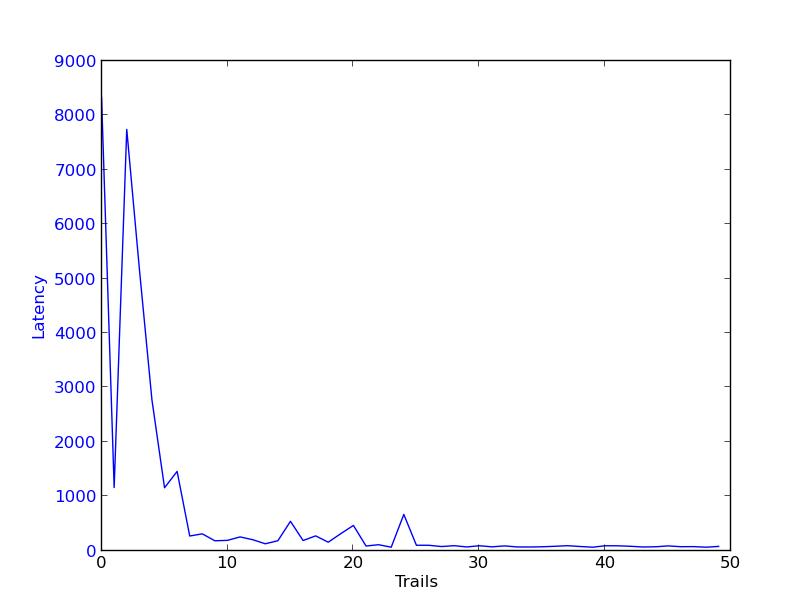
\includegraphics[scale=0.3]{../figure/eps2.jpeg}
      \caption{$\epsilon = 0.2$}
  \end{minipage}%
  \begin{minipage}[c]{0.5\textwidth}
    \centering
    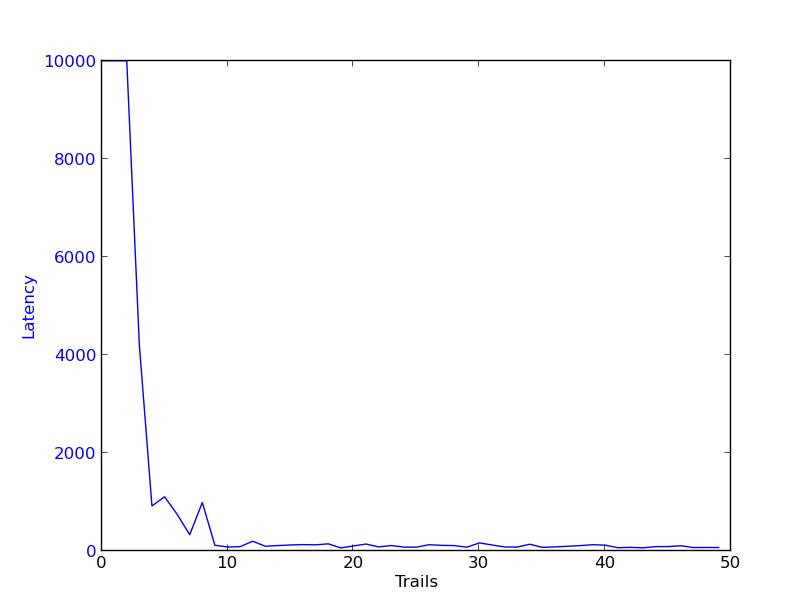
\includegraphics[scale=0.3]{../figure/eps4.jpeg}
      \caption{$\epsilon = 0.4$}
    \end{minipage}
    \\
  \centering
  \begin{minipage}[c]{0.5\textwidth}
    \centering
    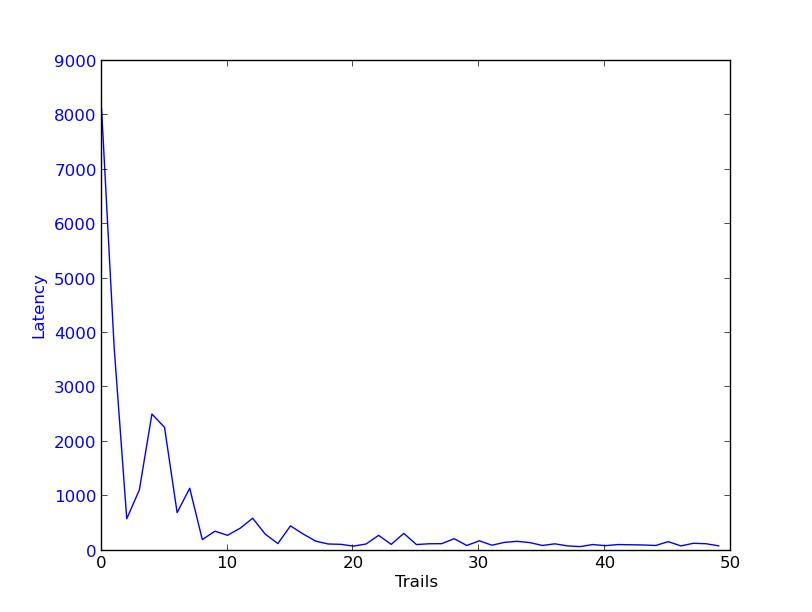
\includegraphics[scale=0.3]{../figure/eps6.jpeg}
  \caption{$\epsilon = 0.6$}
  \end{minipage}%
  \begin{minipage}[c]{0.5\textwidth}
    \centering
    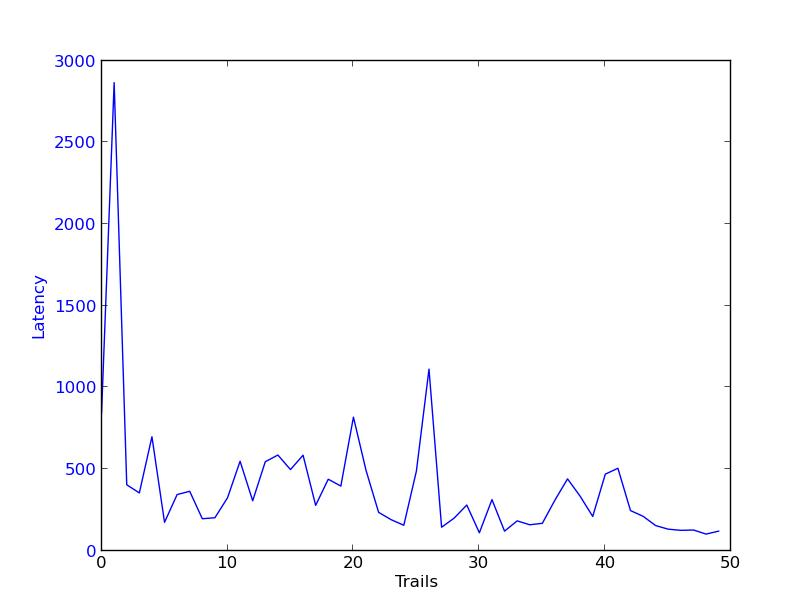
\includegraphics[scale=0.3]{../figure/eps8.jpeg}
  \caption{$\epsilon = 0.8$}
  \end{minipage}
\end{figure}


$\epsilon$ = 0.8 $\Rightarrow$ 219 steps

$\epsilon$ = 0.6 $\Rightarrow$ 113 steps

$\epsilon$ = 0.4 $\Rightarrow$ 77  steps

$\epsilon$ = 0.2 $\Rightarrow$ 79 steps

The result is exactly what we expected. When $\epsilon$ equals to 0.8, the agent quickly finish the first trail (2000 steps average), but it takes more steps in the end, due to the more random choice of the next step. For the small ones, it takes 9000 steps to get to the goal at the begining, but the final averge step is less.

\section{Navigation Map}


The naviagation map is shown as below:

\begin{figure}
  \centering
  \begin{minipage}[c]{0.5\textwidth}
    \centering
    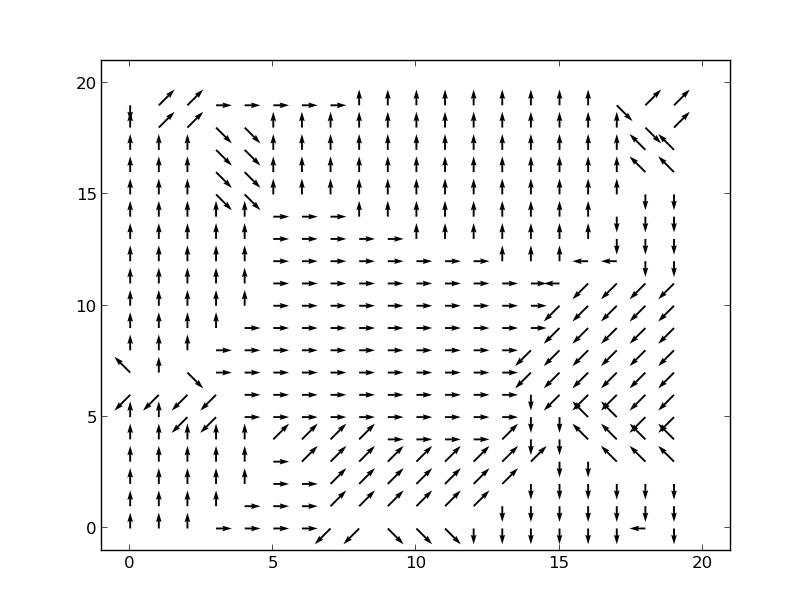
\includegraphics[scale=0.3]{../figure/navMp10.jpeg}
      \caption{Navigation map after 10 steps}
  \end{minipage}%
  \begin{minipage}[c]{0.5\textwidth}
    \centering
    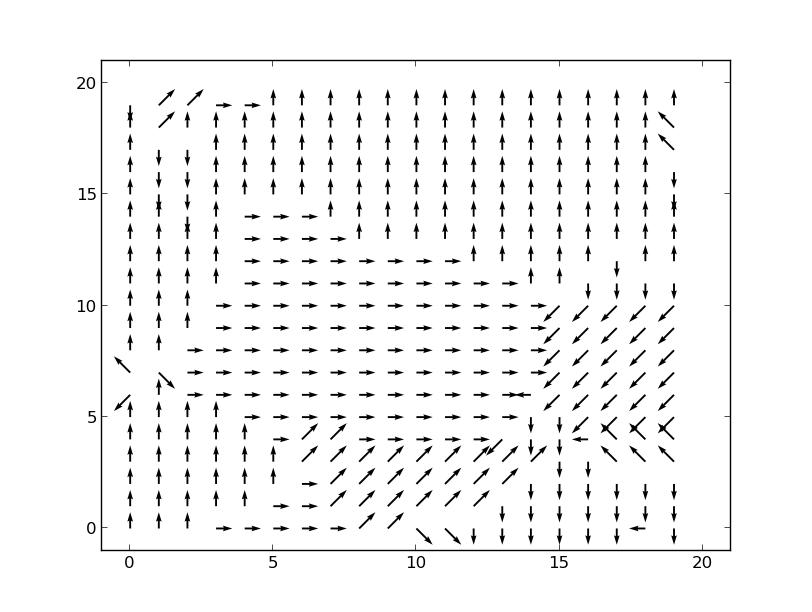
\includegraphics[scale=0.3]{../figure/navMp30.jpeg}
      \caption{Navigation map after 30 steps}
    \end{minipage}
    \\
  \centering
  \begin{minipage}[c]{0.5\textwidth}
    \centering
    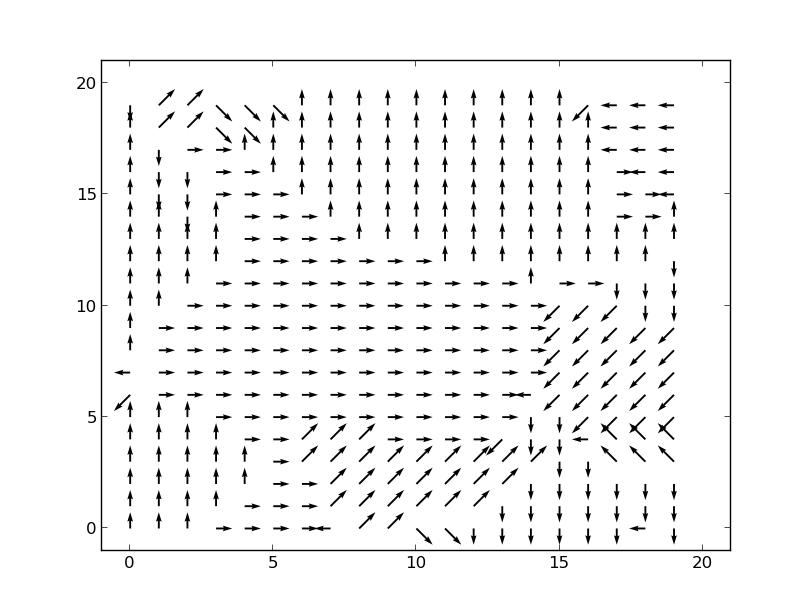
\includegraphics[scale=0.3]{../figure/navMp50.jpeg}
  \caption{Navigation map after 50 steps}
  \end{minipage}%
  \begin{minipage}[c]{0.5\textwidth}
    \centering
    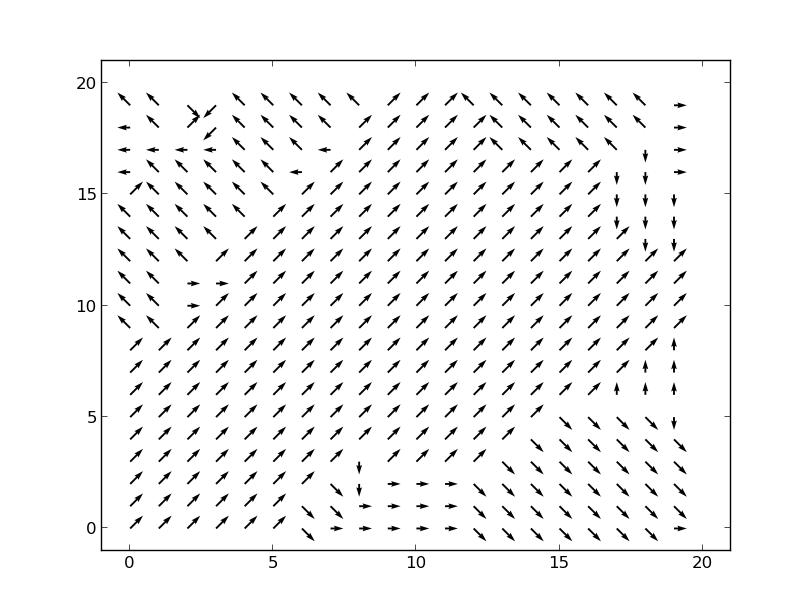
\includegraphics[scale=0.3]{../figure/navMap.jpeg}
  \caption{Best navigation map}
  \end{minipage}
\end{figure}

\end{document}